\lab{Algorithms}{Limitations of Floating Point Computation}{Limitations of Floating Point Computation}
\label{lab:breakfloat}
\objective{Understand the limitations of floating point numbers and introduce numerical stability.}

\section*{Introduction}

In the last lab we discussed the structure and flexibility of floating point numbers.
Floating point numbers are a remarkably versatile tool for performing computations that roughly approximate operations on real numbers.
In this lab we will see how the imperfections of floating point numbers can lead to all kinds of trouble.
There are a variety of common errors involved with floating point computations.
In order to safely use floating point computations it is necessary to know what their limitations are.

We will start by considering a simple example in Cython:

\begin{lstlisting}
cimport numpy as np
def breakfloat(int n):
    cdef np.float32_t a = 2<<26
    cdef int i
    actual = float(a) + n
    for i in range(n):
        a += 1
    return a, actual
\end{lstlisting}

When we run this code for \li{n=2**26} we see that the actual answer is double the answer returned by adding 1 repeatedly.
This is because the floating point number is large enough that adding 1 to it is, after rounding, equivalent to adding 0.
This is effect is mitigated substantially by the use of double precision floating point numbers, but it is still a worry.

\begin{problem}
consider the cython function defined below
\begin{lstlisting}
from numpy cimport ndarray as ar
cimport numpy as np
import numpy as np
from numpy.random import rand
def sumrand(int size, int number):
    # takes the sum of <number> of random arrays
    # with number of elements <size>
    cdef np.float32_t tot=0.
    cdef ar[np.float32_t] A = np.empty(size, dtype=np.float32)
    cdef int i, j
    for i in xrange(number):
        A[:] = rand(size).astype(np.float32)
        for j in xrange(size):
            tot += A[j]
    return tot
\end{lstlisting}
The function call \li{breakfloat2(10**6, 10**3)} returns 16777216.0.
The answer should obviously be around 500000000.
Why is there such a large error?
How could you fix the function so that it would give the right result?
\end{problem}

\section*{Various Computational Considerations}

There are a wide variety of issues that must be considered when using floating point numbers.
Here we will consider a few examples.

The first thing to notice is that floating point numbers are not actually stored as decimal representations.
When you define a decimal number, your computer does the best it can to \emph{approximate} the decimal number given.
For example, when you give your computer a value of .1, the value it actually stores is 0.1000000000000000055511151231257827021181583404541015625 which is usually close enough to .1 that the difference goes unnoticed.
This is, in a sense, a sort of round off error.
These sort of errors can pop up in all kinds of places.
You must also keep in mind that rounding occurs after each operation.
These two effects can combine to give unexpected results, for example
\begin{lstlisting}
>>> 3. * .1 - .3
5.551115123125783e-17
>>> 3. * .1 == .3
False
\end{lstlisting}
These sorts of effects can combine to give somewhat astonishing results, for example, all of the following should be equivalent.
They should all evaluate to 0.
\begin{lstlisting}
>>> n = 19000001
>>> (5*n)**2 - (4*n)**2 - (3*n)**2 # exact result using integers
0
>>> (5.*n)**2 - (4*n)**2 - (3*n)**2 # added a single decimal point
1.0
>>> (5*n)**2 - (4.*n)**2 - (3*n)**2 # added a single decimal point somewhere else
-1.0
>>> (5.*n)**2 - ((4*n)**2 + (3*n)**2) # added a decimal point and some parenthesis
2.0
\end{lstlisting}
Notice how four expressions that should, in theory, be equivalent returned four \emph{different} answers.
The change caused by the inclusion of parenthesis is particularly troublesome because it means that floating point operations are only \emph{approximately} associative.
This is an example of what is called catastrophic cancellation.
Catastrophic cancellation occurs when we perform an operation on two floating point numbers that are already subject to rounding error.
it is especially noticeable when subtracting numbers that are approximately equal.
Because different methods of computation may yield slightly different results it is imperative that equality tests and comparisons using floating point numbers be carried out with certain tolerances.
It is all too tempting to do some floating point computation that you would expect to give a result of 0 and then to test your result with something like
\begin{lstlisting}
if result == expected:
    print "it worked"
\end{lstlisting}
and then try to debug a perfectly good bit of code because the way it does its computations gives a result that is minutely different than what you expect.
A test like this should be replaced with something roughly along the lines of
\begin{lstlisting}
tolerance = 1E-6
if abs(result - expected) < tolerance:
    print "it worked"
\end{lstlisting}
For a specific example, consider the square root function given in the previous lab for 32 bit floating point numbers.
The square root given is not a perfect match to the square root given by the built in square root function, but it can compute the proper value so that all but the last bit is accurate.
To test whether or not the algorithm converges for randomly generated numbers between 0 and 1 we may be tempted to do the following
\begin{lstlisting}
A = rand(10000)
(pysqrtacc32(A, 2) == np.sqrt(A)).all()
\end{lstlisting}
Which would return \li{False} since some of the values returned by our \emph{algorithm} may differ from the built in square root by an extremely small amount regardless of how many iterations we run.
We can test for accuracy properly using something like
\begin{lstlisting}
A = rand(10000)
(np.absolute(pysqrtacc32(A, 2) - np.sqrt(A)) < 2E-7).all()
\end{lstlisting}
Which returns \li{True}.

\begin{problem}
One example where it is common to subtract numbers that are nearly equal is in the computation of numerical derivatives.
Write a simple approximation to the derivative of a function $f$ using the formula $\frac{f(x+h) - f(x)}{h}$.
Check how accurate it is for varying sizes of \li{h} by testing it on the \li{sin} function included in Python's math library with \li{x = 1}.
Use Python's \li{cos} function as the exact value of the derivative.
What do you notice about accuracy as \li{h} becomes smaller and smaller?
\end{problem}

\begin{figure}
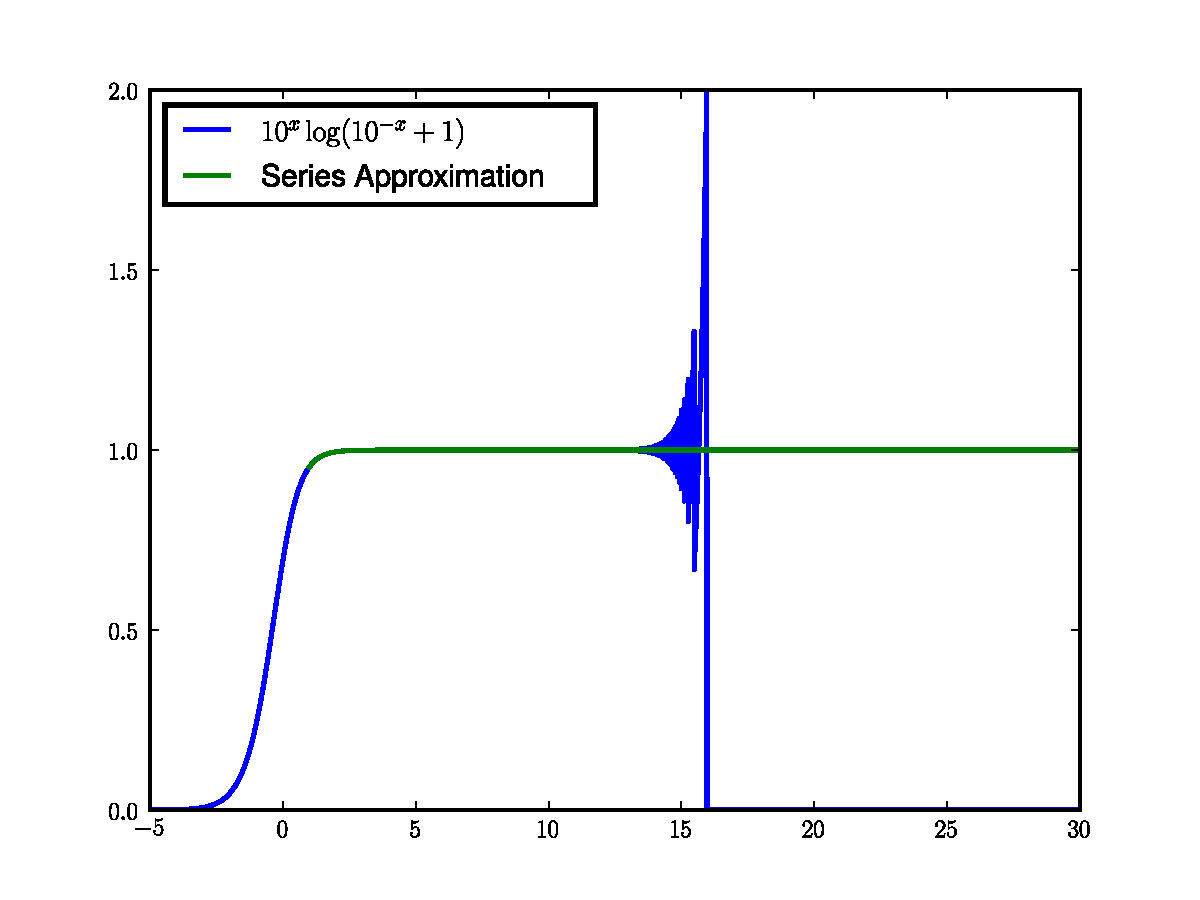
\includegraphics[width=\textwidth]{lnseries.pdf}
\caption{Floating point computation of $\frac{\ln \left(x+1\right)}{x}$ shown with a corresponding series approximation.}
\label{floatbreak:lnseries}
\end{figure}

\begin{problem}
Sometimes clever numerical methods can be used to avoid some of the issues involved in floating point computations.
The value for $\frac{\ln \left(x+1\right)}{x}$ can be approximated by the series
\[
\sum_{n=1}^{\infty} \frac{\left( -1 \right)^{n+1}}{n} x^n
\]
where $\| x \| \leq 1$.
Use this series to obtain a more accurate approximation of $\frac{\ln \left(x+1\right)}{x}$ for extremely small floating point numbers.
Using the polynomial you have constructed plot the exact value and the approximation to the function $ln \left( 10^{-x} + 1 \right)10^{x}$.
Plot the exact value on $[-5, 30]$.
Plot the approximation on $[1, 30]$.
Your plot should look roughly like the plot shown in Figure \ref{floatbreak:lnseries}.
\end{problem}

Another limitation of floating point numbers is that they are subject to overflow.
Floating point numbers do have restricted values set aside for values of $\infty$, $-\infty$, and \li{Nan}, so you can often tell when overflow has occured, but it is best to avoid extremely large or extremely small floating point values in either case.
For a simple example of overflow, we will perform a computational demonstration that the $p$-norms approach the $\infty$-norm as $p \rightarrow \infty$.
\begin{lstlisting}
def pnorm(A, p):
    return (A**p).sum()**(1./p)
\end{lstlisting}
If you haven't seen p-norms before, the main thing you need to understand here is that as $p \rightarrow \infty$, \li{pnorm(A, p)} should come arbitrarily close to \li{np.absolute(A).max()}.
Testing this computationally, we see that, for a randomly generated array of values between 0 and 1, we get the plot shown in Figure \ref{pnorm_convergence} as $p \rightarrow \infty$.

\begin{figure}
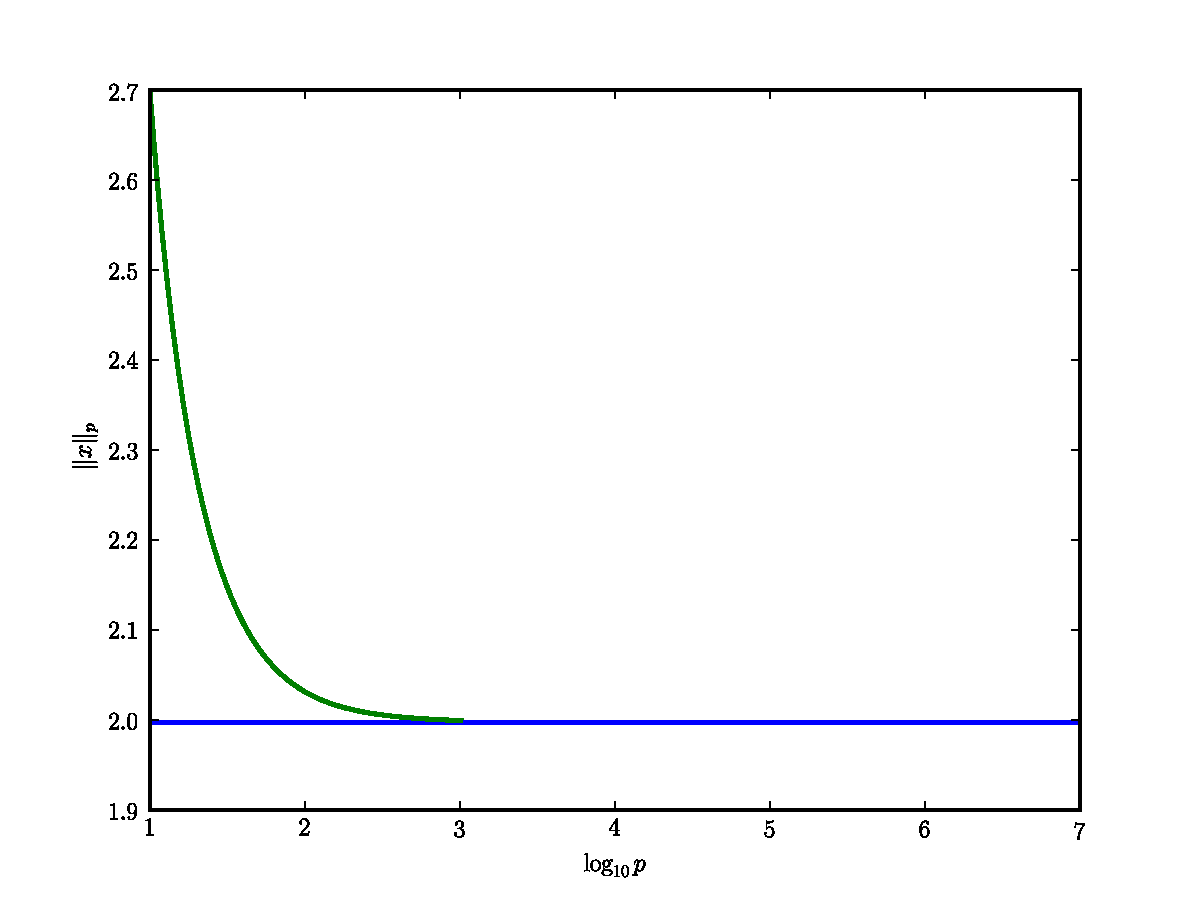
\includegraphics[width=\textwidth]{pnorm_convergence.pdf}
\caption{The convergence of the $p$-norms to the $\infty$-norm for a randomly generated vector of 100 floating point values in $(1,2)$.
Notice how the $p$-norms disappear when $p$ is roughly 1000.
This is because values of floating point infinity are introduced into the computation.
This is especially troublesome because the array is nearly at the middle of the range of possible floating point values.
If the maximum were less than 1, the norm would suddenly drop to zero instead of jumping to $\infty$.}
\label{pnorm_convergence}
\end{figure}

For floating point numbers, overflow results in a value of $\infty$ or $-\infty$.
Operations that cannot be well defined (like $\infty - \infty$) return a value of \li{NAN}, which stands for "Not A Number."
When dealing with machine integers, for example integers that are stored in arrays or integers in programming languages other than Python, there are no specific values for things likt $\infty$.
The operations can be performed, but the result will be incorrect.
To understand this, first consider an unsigned integer.
Unsigned integers are always considered to be positive.
Unsigned integers have no sign, so each bit is considered a binary digit.
In an eight bit unsigned integer there are 256 possible values.
They are used to represent the numbers 0 through 255.
When we pass 255, the numbers cycle back around to 0 again, so, for example:
\begin{lstlisting}
>>> np.arange(250, 260, dtype=np.uint8)
array([250, 251, 252, 253, 254, 255,   0,   1,   2,   3], dtype=uint8)
>>> np.arange(250, 260, dtype=np.uint8) * 2
array([244, 246, 248, 250, 252, 254,   0,   2,   4,   6], dtype=uint8)
>>> np.arange(250, 260, dtype=np.uint8)**2
array([36, 25, 16,  9,  4,  1,  0,  1,  4,  9], dtype=uint8)
\end{lstlisting}
As you can see, the operations can be understood as operations in $\mathbb{Z} / 256 \mathbb{Z}$, which has operations equivalent to those in $\mathbb{Z}$ only some of the time.
These sorts of issues can come up in computations involving integers or even typecasts to integers.

% this is another possibly useful problem, but it can be removed if necessary
\begin{problem}
Your friend writes the following Cython code to search for Pythagorean Triples.
\begin{lstlisting}
from libc.math cimport sqrt
def find_triple(double start, int num):
    cdef int i, j
    cdef double temp
    for i in xrange(num):
        for j in xrange(i, num):
            temp = sqrt((start+i)**2 + (start+j)**2)
            if temp == int(temp):
                print int(start+i), int(start+j), int(temp)
\end{lstlisting}
By running \li{find_triple(600000000, 10000)}, he claims to have found the triples

600001807  600004043  848532274

600001924  600004742  848532851

600004561  600009787  848538283

600004738  600007261  848536622

{\setlength{\parindent}{0cm}
What is wrong with his code and how should it be fixed?
Be sure to watch out for any integer overflow along the way.
}
\end{problem}

\section*{Some Examples of Computation Error}

There have been several historical examples where incorrect numerical computing has caused terrible disasters.

Our first example involves the explosion of the Ariane 5 rocket in 1996.
The Ariane 5 rocket was launched by the European Space Agency.
Roughly 7 billion dollars were spent in its development.
The rocket and its cargo were, in themselves, worth an estimated 500 million dollars.
At an altitude of about 3700 meters the rocket veered off of its intended path and exploded.
After some investigation it was discovered that the error was caused by the conversion of an excessively large 64 bit floating point number to a 16 bit signed integer.
To see how this could cause problems, consider the following example:
\begin{lstlisting}
>>> from numpy.random import rand
>>> A = rand(10) * 10**5
>>> A.astype(np.int16) # incorrect cast, overflow has occured
array([  6691,  24236, -28341,   4104,  18063, -19080,  -7500,  -4954,
        25898,  11995], dtype=int16)
>>> A.astype(np.int64) # what the values should be
array([26802, 64425,  1339, 55901, 51665, 11992, 90368, 87717,    25, 38894], dtype=int64)
\end{lstlisting}
Keep in mind that a simple error like this caused hundreds of millions of dollars of damage.

The Vancouver Stock Exchange is another example of a relatively simple propagation of error.
When the exchange opened, the index to track its value was initialized at 1000 in January of 1982.
Around 3000 times per day the index was updated and then truncated to three decimals of precision.
After 22 months the computed value was 524.881 when the actual value should have been 1009.811.
When it was discovered that the computation of the index was diminishing it's value, the index was reset to its actual value.

Another example which we will not discuss here was the sinking of the Sleipner A offshore platform in 1991.
That disaster was due to improper finite element analysis.
The total loss was estimated at 700 million dollars.

The final example we will consider here is the failure of the Patriot Missile Defense system at Dharan, Saudi Arabia during the gulf war.
In this disaster the patriot missile system failed to fire on an incoming missile.
The missile struck a barracks, killed 28 people, and injured around 100 others.
This failure was due to improper use of floating point numbers!
The system clock was incremented using every .1 seconds using integers, but the time was then converted back to float by multiplying by .1 for use in some floating point computations.
After 100 hours of operation the roundoff error in the floating point representation of .1 became significant enough that it prevented the system from properly targeting an incoming missile.

\begin{problem}
In the floating point format used for the Patriot missile systems in the gulf war the closest floating point number to .1 was $\frac{209715}{2097152}$.
Calculate the error accumulated over 100 hours.
If a missile travels at 1676 meters per second, how far will it be able to travel in that amount of time?
\end{problem}